\section{Experimental results}

In both of our experiments, a toy query, "usa election president politics " was
used. We first tried using only tf-idf and then a combined retrieval with standard 
PageRank, both of which were compared to combined retrieval with our novel PageRank variant, 
which considers how many followers a user has. We graded the top ten results of each retrieval 
as relevant or not and plotted aprecision vs recall graph for each of them.

\subsection{TF-IDF}

\begin{figure}[H]
\centering
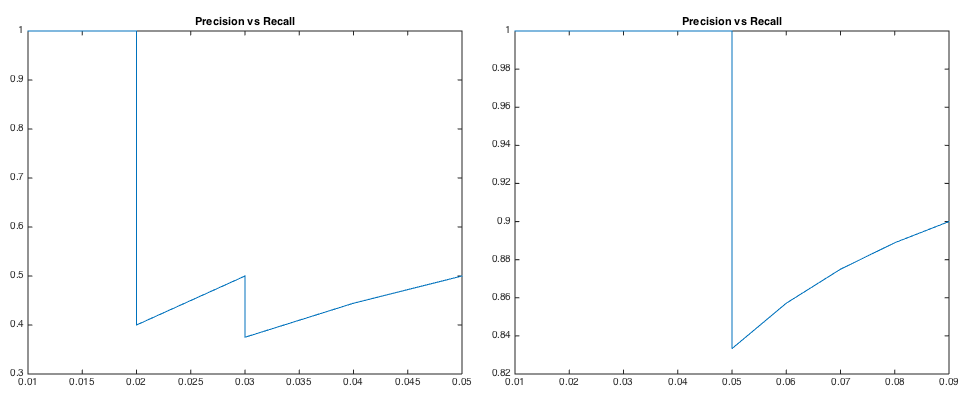
\includegraphics[width=5.5in,natwidth=534,natheight=345]{images/exptfidf.png}
\caption{Precision vs Recall for TF-IDF only (left) and combination with PageRank based on the number of followers ($\alpha = 0.5$).}
\label{fig:exptfidf}
\end{figure}

As expected, a combination of TF-IDF with PageRank performs better than just the
first algorithm.  The problem is that our database does not contain \emph{all}
the tweets of each user, so the bag of words model is only precise among the
crawled topics. If, for instance, a user posts a single tweet about politics and
we only crawl that tweet for that user, it's going to appear really well-ranked
for TF-IDF while, in reality, it shouldn't. When PageRank is added to the
equation we exploit the graph structure of Twitter and take the authority of the
aforementioned user in consideration, which highly improves our Precision vs
Recall curve, as can be seen in Figure \ref{fig:exptfidf}.

\subsection{Standard PageRank}

\begin{figure}[H]
\centering
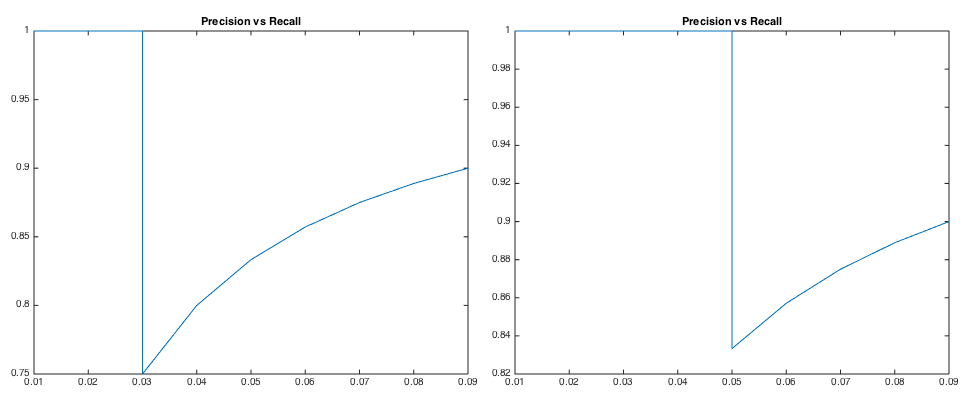
\includegraphics[width=5.5in,natwidth=966,natheight=420]{images/exptopr.png}
\caption{Precision vs Recall for PageRank using the classic algorithm (left) and the one based on the number of followers.}
\label{fig:exptopr}
\end{figure}

In Figure \ref{fig:exptopr} we use two different methods for PageRank: the
classic method where the jump between mentions of a user is done with equal
probabilities, and using higher chance of jumping based on the number of
followers. As we can see, the precision-at-10 of our novel method is
considerably better than using the classic algorithm, and we attribute that to
the nature of our problem: since our engine is recommending users to follow,
users with high number of followers can be considered as good candidates.
However, using this extensively may result in recommending the same top users
always, which may end up penalizing too much relevant but unpopular users or the
ones which are new in Twitter.
